\documentclass[]{article}
\usepackage[]{newpxtext,newpxmath,inconsolata}
\usepackage{amssymb,amsmath}
\usepackage{ifxetex,ifluatex}
\usepackage{fixltx2e} % provides \textsubscript
\ifnum 0\ifxetex 1\fi\ifluatex 1\fi=0 % if pdftex
  \usepackage[T1]{fontenc}
  \usepackage[utf8]{inputenc}
\else % if luatex or xelatex
  \ifxetex
    \usepackage{mathspec}
  \else
    \usepackage{fontspec}
  \fi
  \defaultfontfeatures{Ligatures=TeX,Scale=MatchLowercase}
\fi
% use upquote if available, for straight quotes in verbatim environments
\IfFileExists{upquote.sty}{\usepackage{upquote}}{}
% use microtype if available
\IfFileExists{microtype.sty}{%
\usepackage{microtype}
\UseMicrotypeSet[protrusion]{basicmath} % disable protrusion for tt fonts
}{}
\usepackage[margin=1in]{geometry}
\usepackage{hyperref}
\hypersetup{unicode=true,
            pdftitle={Neurotechnology+0001},
            pdfauthor={Slap Fingerprint Segmentation Evaluation III},
            pdfborder={0 0 0},
            breaklinks=true}
\urlstyle{same}  % don't use monospace font for urls
\usepackage{longtable,booktabs}
\usepackage{graphicx,grffile}
\makeatletter
\def\maxwidth{\ifdim\Gin@nat@width>\linewidth\linewidth\else\Gin@nat@width\fi}
\def\maxheight{\ifdim\Gin@nat@height>\textheight\textheight\else\Gin@nat@height\fi}
\makeatother
% Scale images if necessary, so that they will not overflow the page
% margins by default, and it is still possible to overwrite the defaults
% using explicit options in \includegraphics[width, height, ...]{}
\setkeys{Gin}{width=\maxwidth,height=\maxheight,keepaspectratio}
\IfFileExists{parskip.sty}{%
\usepackage{parskip}
}{% else
\setlength{\parindent}{0pt}
\setlength{\parskip}{6pt plus 2pt minus 1pt}
}
\setlength{\emergencystretch}{3em}  % prevent overfull lines
\providecommand{\tightlist}{%
  \setlength{\itemsep}{0pt}\setlength{\parskip}{0pt}}
\setcounter{secnumdepth}{5}
% Redefines (sub)paragraphs to behave more like sections
\ifx\paragraph\undefined\else
\let\oldparagraph\paragraph
\renewcommand{\paragraph}[1]{\oldparagraph{#1}\mbox{}}
\fi
\ifx\subparagraph\undefined\else
\let\oldsubparagraph\subparagraph
\renewcommand{\subparagraph}[1]{\oldsubparagraph{#1}\mbox{}}
\fi

%%% Use protect on footnotes to avoid problems with footnotes in titles
\let\rmarkdownfootnote\footnote%
\def\footnote{\protect\rmarkdownfootnote}

%%% Change title format to be more compact
\usepackage{titling}

% Create subtitle command for use in maketitle
\providecommand{\subtitle}[1]{
  \posttitle{
    \begin{center}\large#1\end{center}
    }
}

\setlength{\droptitle}{-2em}

  \title{\texttt{Neurotechnology+0001}}
    \pretitle{\vspace{\droptitle}\centering\huge}
  \posttitle{\par}
  \subtitle{Neurotechnology}
  \author{Slap Fingerprint Segmentation Evaluation III}
    \preauthor{\centering\large\emph}
  \postauthor{\par}
      \predate{\centering\large\emph}
  \postdate{\par}
    \date{Last Updated: 08 May 2019}

\usepackage{fancyhdr}
\usepackage[table]{xcolor}
\newcommand{\algorithm}{Neurotechnology+0001}
\lhead{\texttt{\algorithm}}
\chead{\textsc{\small Slap Fingerprint Segmentation III Report Card}}
\rhead{\thepage}
\lfoot{}
\cfoot{}
\rfoot{}
\renewcommand{\headrulewidth}{1pt}
\pagestyle{fancy}

\begin{document}
\maketitle

{
\setcounter{tocdepth}{2}
\tableofcontents
}
\clearpage

\section{Participation Information}\label{participation-information}

\subsection{Names and Dates}\label{names-and-dates}

\begin{itemize}
\tightlist
\item
  \textbf{Organization Name:} Neurotechnology
\item
  \textbf{SlapSeg III Identifier:} \texttt{Neurotechnology+0001}
\item
  \textbf{Provided Marketing Name:} ``MegaMatcher''
\item
  \textbf{Application Date:} 27 February 2019
\item
  \textbf{First Submission Date:} 29 April 2019 (as version
  \texttt{0000})
\item
  \textbf{Validation Date:} 08 May 2019
\item
  \textbf{Completion Date} 08 May 2019
\end{itemize}

\subsection{Libraries}\label{libraries}

\begin{table}[!h]
\centering
\begin{tabular}{lll}
\toprule
Filename & MD5 Checksum & Size\\
\midrule
\rowcolor{gray!6}  Fingers.ndf & \ttfamily{2c64094f25b2e21c692d9ee1c38da3cb} & 1.5 Mb\\
libinference\_engine.so & \ttfamily{b5f030ca684a4ff4e75bc81b526b5dd2} & 4.1 Mb\\
\rowcolor{gray!6}  libiomp5.so & \ttfamily{2729cb28f53ff764c280a30474e10bea} & 2 Mb\\
libMKLDNNPlugin.so & \ttfamily{26f184987694185b14d3cdd15005d92a} & 13.9 Mb\\
\rowcolor{gray!6}  libmkl\_tiny\_omp.so & \ttfamily{2970e5c3f5154ad7c13b3136736143e0} & 26.6 Mb\\
libslapsegiii\_Neurotechnology\_0001.so & \ttfamily{f586c7a338c6d120e7129f914f25d0a7} & 10.1 Mb\\
\bottomrule
\end{tabular}
\end{table}

\clearpage

\section{\texorpdfstring{Tenprint Cards (``TwoInch''
Data)}{Tenprint Cards (TwoInch Data)}}\label{tenprint-cards-twoinch-data}

\subsection{Segmentation Timing}\label{segmentation-timing}

All algorithms are run over a small fixed corpus of TwoInch images to
estimate the total runtime of the evaluation. To be evaluated under
SlapSeg III, algorithms \textbf{must} segment the timing corpus, on
average, in under \(1\,500\) milliseconds. This maximum reference time
is documented in the SlapSeg III test plan, and is subject to change.

Box plots of segmentation times are separated by slap orientation and
capture technology in
\protect\hyperlink{fig:fig-twoinch-timing-tex}{Figure
\ref{fig:fig-twoinch-timing-tex}}. Tabular representations are
enumerated in \protect\hyperlink{tab:tab-twoinch-timing}{Table
\ref{tab:tab-twoinch-timing}}. Results are reported in milliseconds.

\begin{figure}[h]

{\centering 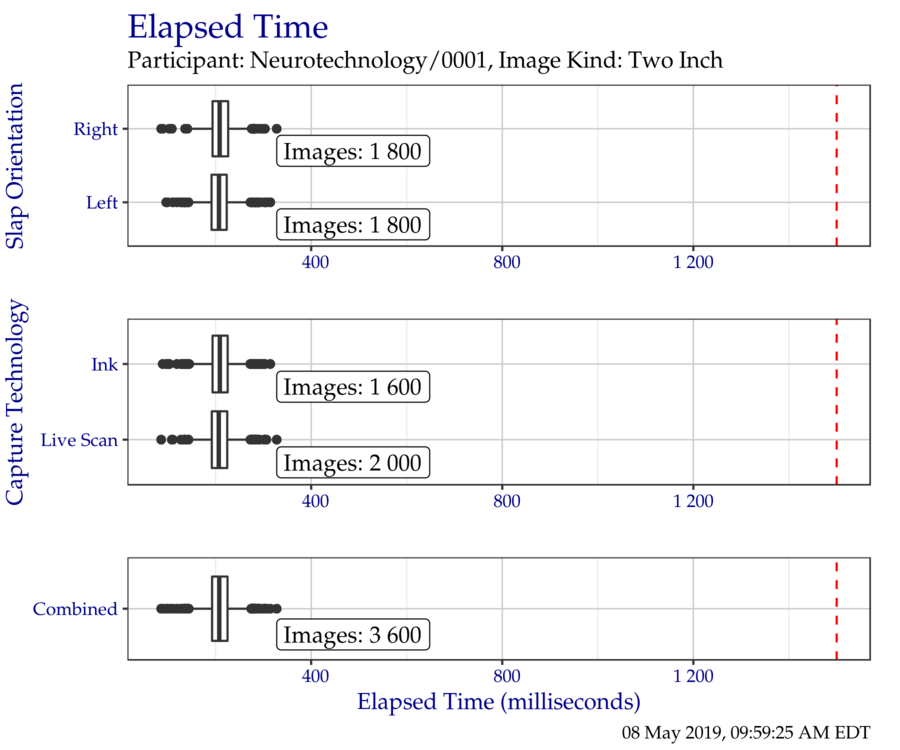
\includegraphics[height=320px]{/mnt/isiA01/evaluations/slapsegiii/analysis/intermediate/Neurotechnology/0001/timing/Neurotechnology+0001_timing_TwoInch_timing} 

}

\caption{Box plots of elapsed time in milliseconds when segmenting the TwoInch timing test corpus, separated by slap orientation and capture technology.}\label{fig:fig-twoinch-timing-tex}
\end{figure}

\begin{table}[!h]

\caption{\label{tab:tab-twoinch-timing}Elapsed time in milliseconds when segmenting the TwoInch timing test corpus, separated by slap orientation and capture technology.}
\centering
\begin{tabular}{lr>{}r|r>{}r|r}
\toprule
 & Right & Left & Live Scan & Ink & Combined\\
\midrule
\rowcolor{gray!6}  Minimum & 86 & 97 & 86 & 89 & 86\\
25\% & 194 & 191 & 192 & 194 & 193\\
\rowcolor{gray!6}  Median & 208 & 207 & 207 & 209 & 208\\
75\% & 226 & 223 & 224 & 225 & 225\\
\rowcolor{gray!6}  Maximum & 328 & 314 & 328 & 314 & 328\\
\bottomrule
\end{tabular}
\end{table}

\clearpage

\subsection{Segmentation Centers and
Dimensions}\label{segmentation-centers-and-dimensions}

\subsubsection{Segmentation Centers}\label{segmentation-centers}

The plots in this section show the distribution of segmentation position
centers \((x,y)\) for TwoInch data. At the top of each figure is a
combined plot for all finger positions of a given slap orientation.
These figures are isolated in plots faceted at the bottom of the figure.

Plots of segmentation centers for the right hand TwoInch data are shown
in \protect\hyperlink{fig:twoinch-centers-right}{Figure
\ref{fig:twoinch-centers-right}} and plots of segmentation centers for
the left hand are shown in
\protect\hyperlink{fig:twoinch-centers-left}{Figure
\ref{fig:twoinch-centers-left}}. Blank lines that may appear in the
plots are \textbf{not} rendering artifacts. Rather, they are indicative
of image downsampling.

Points in each plot are plotted with a semi-transparent opacity. This
results in points of particular color appearing ``darker'' to indicate a
higher frequency of the observed value, while ``lighter'' points
indicate a lower observed frequency.

\begin{figure}

{\centering 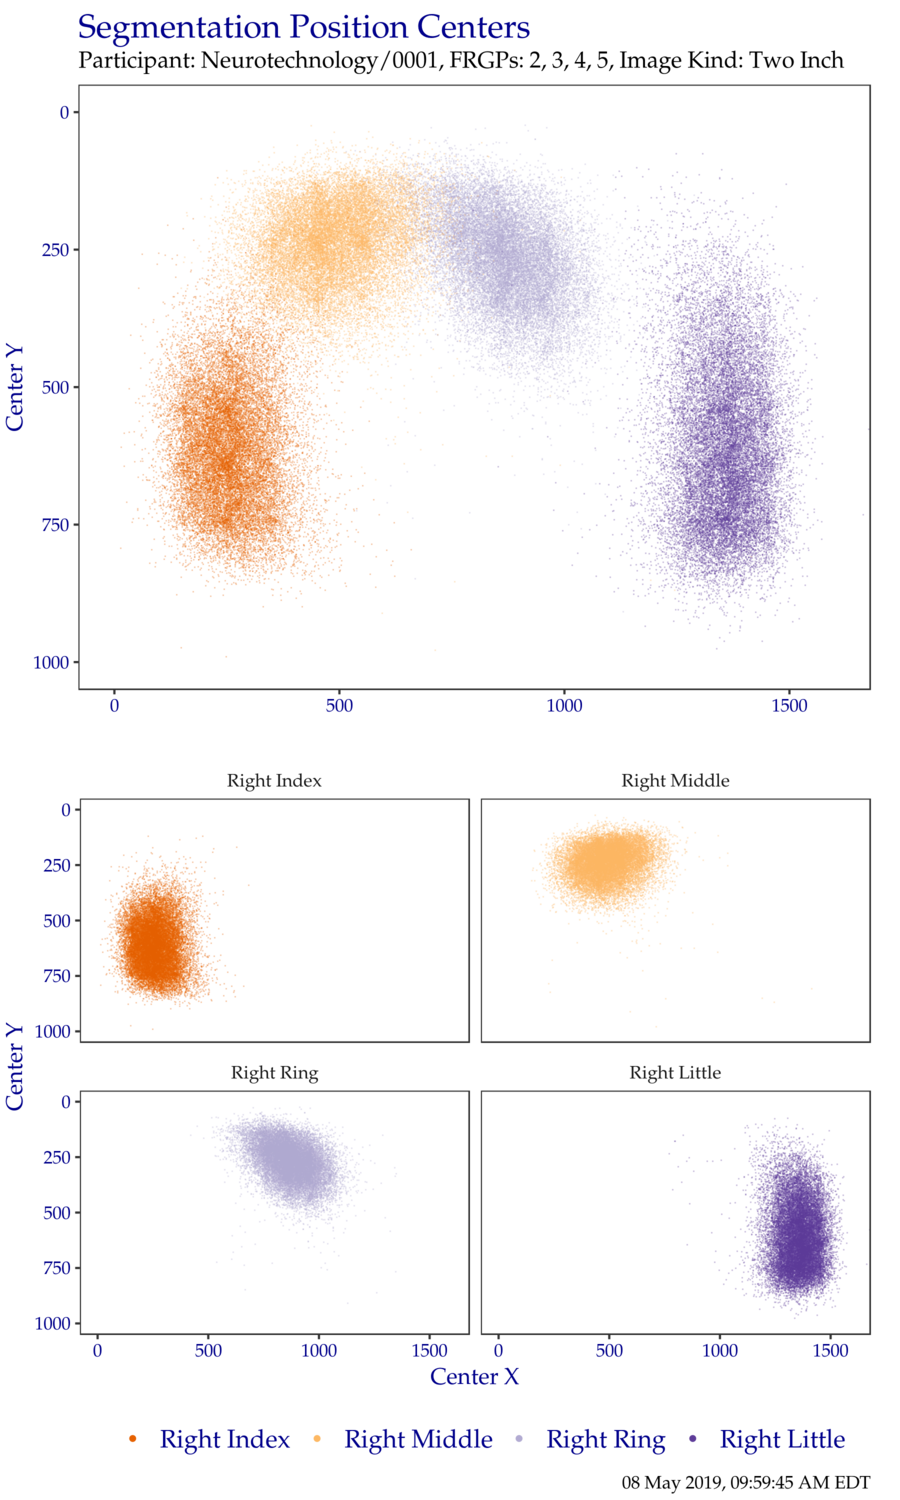
\includegraphics{/mnt/isiA01/evaluations/slapsegiii/analysis/intermediate/Neurotechnology/0001/full/Neurotechnology+0001_full_TwoInch_center_right} 

}

\caption{Segmentation centers for right hand TwoInch data.}\label{fig:twoinch-centers-right}
\end{figure}

\begin{figure}

{\centering 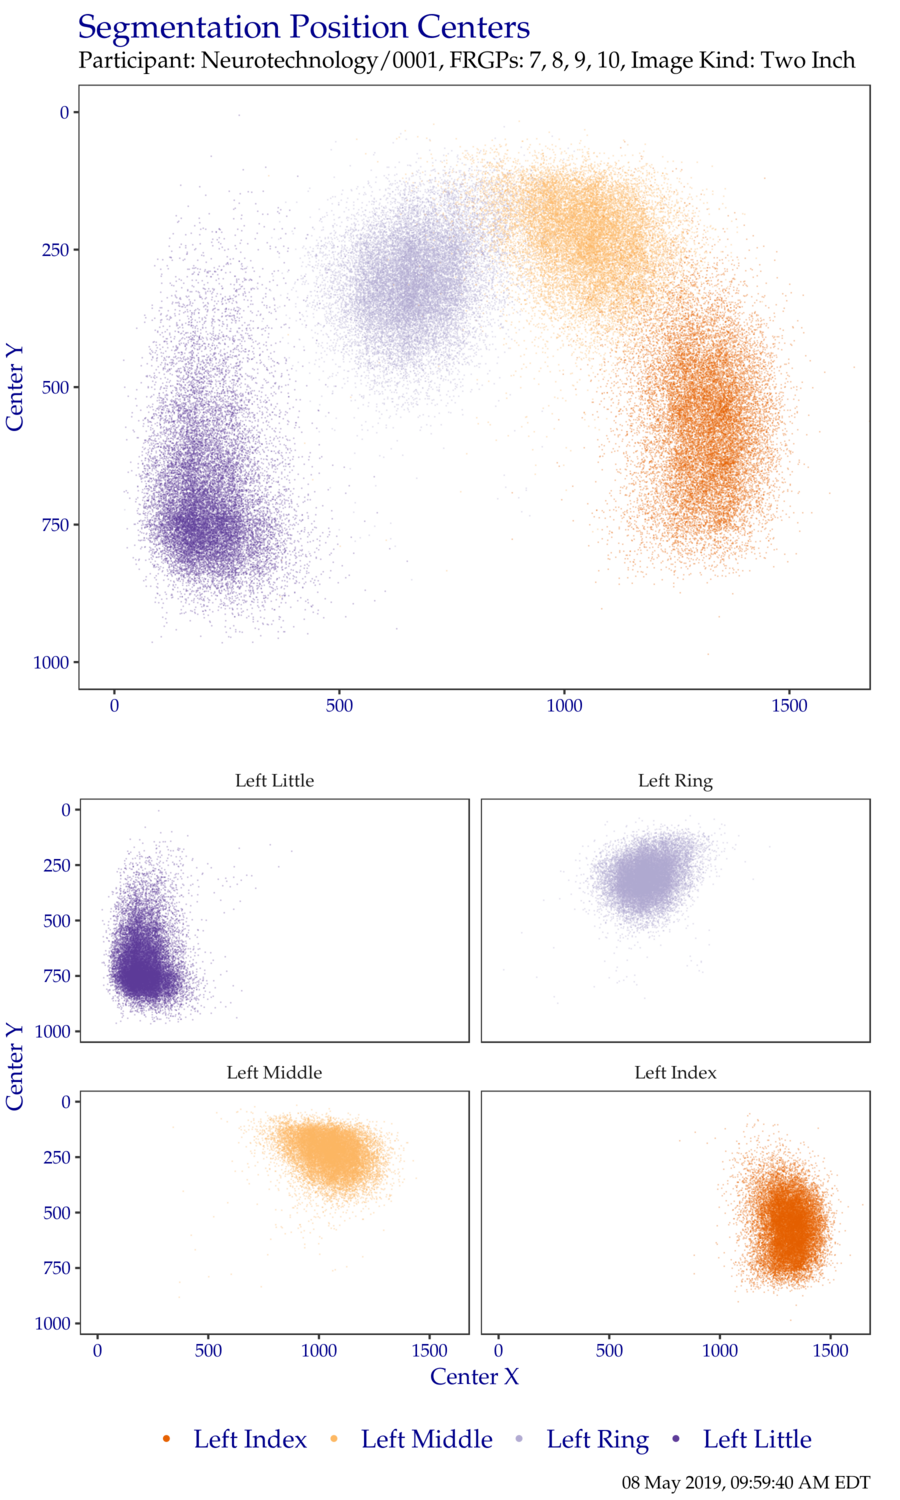
\includegraphics{/mnt/isiA01/evaluations/slapsegiii/analysis/intermediate/Neurotechnology/0001/full/Neurotechnology+0001_full_TwoInch_center_left} 

}

\caption{Segmentation centers for left hand TwoInch data.}\label{fig:twoinch-centers-left}
\end{figure}

\clearpage

\subsubsection{Segmentation Dimensions}\label{segmentation-dimensions}

The plots in this section show the distribution of segmentation position
widths and heights for TwoInch data. At the top of each figure is a
combined plot for all finger positions of a given slap orientation.
These figures are isolated in plots faceted at the bottom of the figure.

Plots of segmentation position dimensions for the right hand TwoInch
data are shown in \protect\hyperlink{fig:twoinch-wh-right}{Figure
\ref{fig:twoinch-wh-right}} and the left hand in
\protect\hyperlink{fig:twoinch-wh-left}{Figure
\ref{fig:twoinch-wh-left}}. Blank lines that may appear in the plots are
\textbf{not} rendering artifacts. Rather, they are indicative of image
downsampling.

\begin{figure}

{\centering 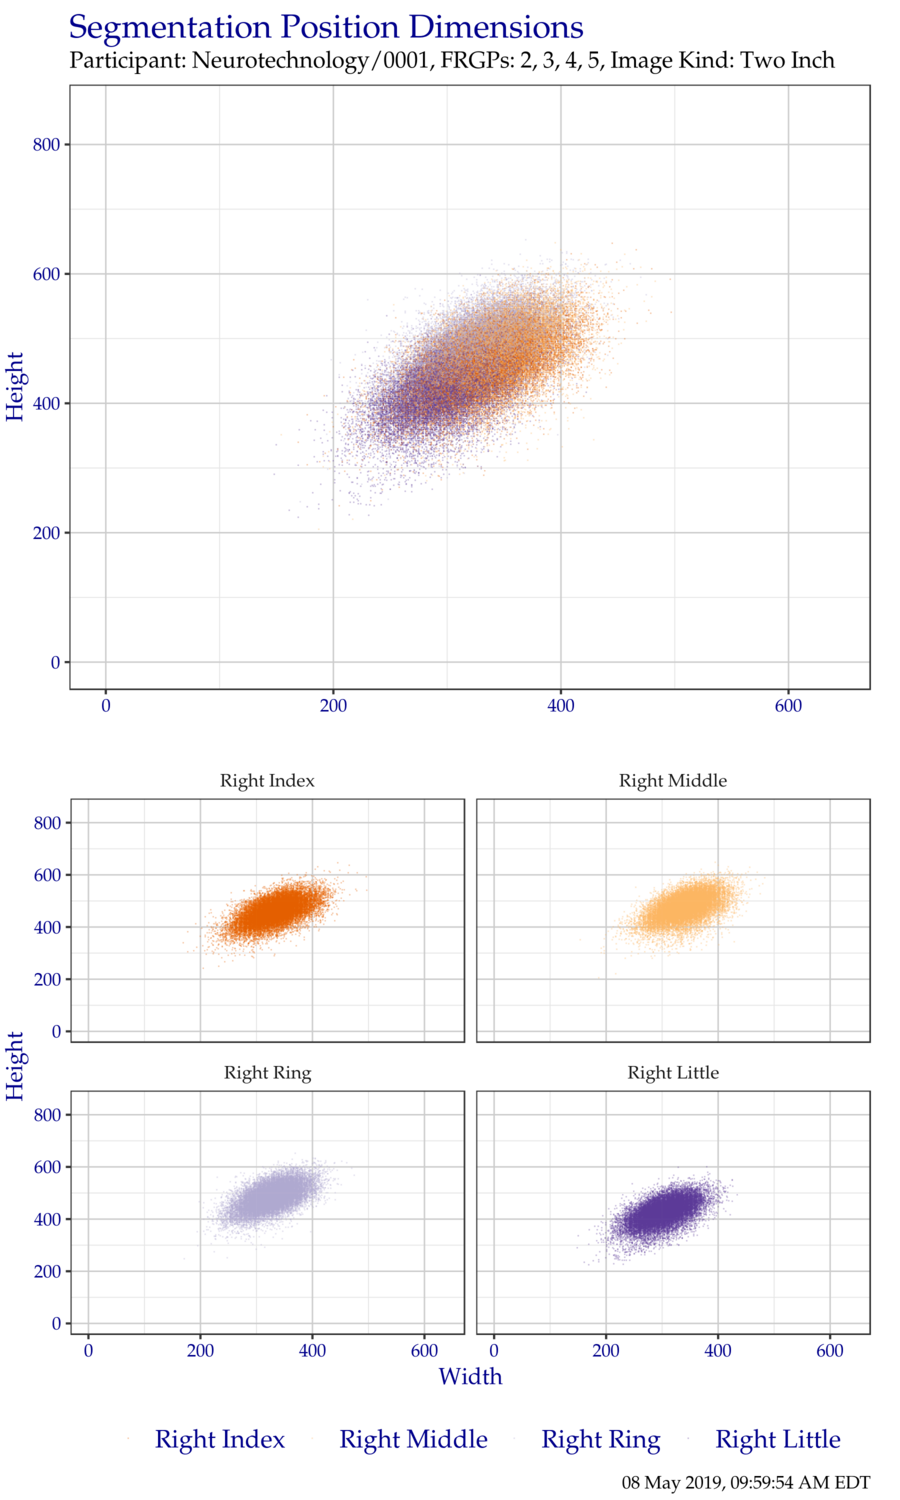
\includegraphics{/mnt/isiA01/evaluations/slapsegiii/analysis/intermediate/Neurotechnology/0001/full/Neurotechnology+0001_full_TwoInch_wh_right} 

}

\caption{Segmentation position dimensions for right hand TwoInch data.}\label{fig:twoinch-wh-right}
\end{figure}

\begin{figure}

{\centering 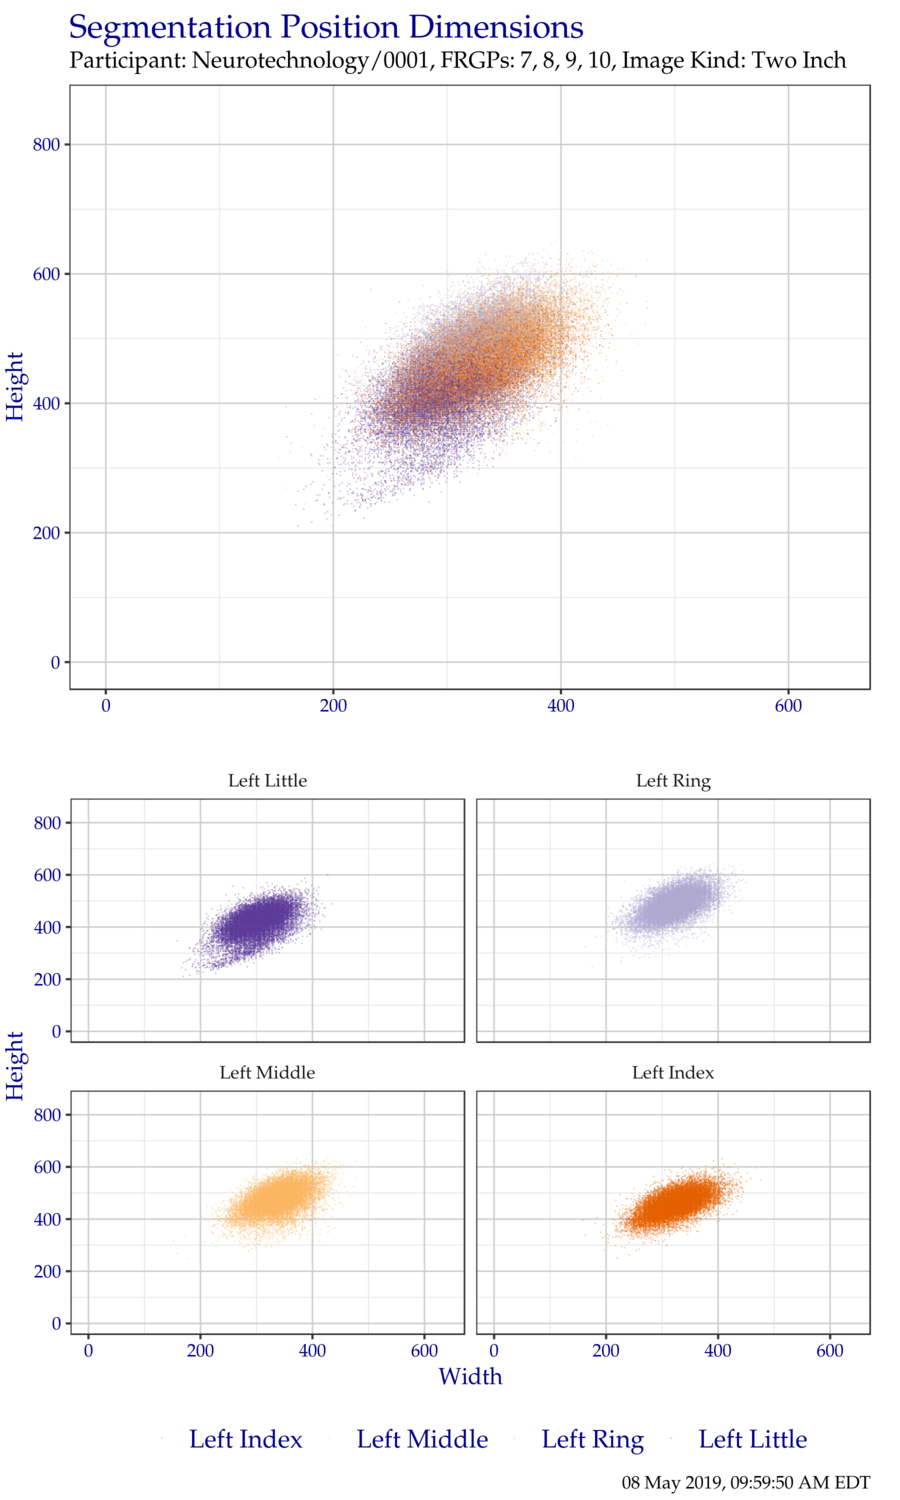
\includegraphics{/mnt/isiA01/evaluations/slapsegiii/analysis/intermediate/Neurotechnology/0001/full/Neurotechnology+0001_full_TwoInch_wh_left} 

}

\caption{Segmentation position dimensions for left hand TwoInch data.}\label{fig:twoinch-wh-left}
\end{figure}

\clearpage

\hypertarget{subsec-twoinch-stats}{\subsection{Detailed Segmentation
Statistics}\label{subsec-twoinch-stats}}

This section shows detailed results of segmentation of TwoInch data.
Values in each table are the percentage that the variable in the
left-most column was correctly segmented.

Each table has three columns of percentages. The \emph{Standard Scoring}
column shows the percentage of correctly-segmented positions based on
the scoring metrics defined in the SlapSeg III scoring document. The
\emph{Ignoring Bottom Y} column shows how the percentage would change if
the threshold for the \emph{bottom} \(Y\) coordinate of the segmentation
position was ignored. Similarly, the \emph{Ignoring Bottom X and Y}
columns shows how the percentage would change if only the top, left, and
right sides of the segmentation position were considered. These two
supplemental columns are included because it has traditionally been
difficult to determine the exact location of the distal interphalangeal
joint.

\protect\hyperlink{twoinch-per-subject}{Table
\ref{tab:twoinch-per-subject}} shows how successful
\texttt{Neurotechnology+0001} segmented fingers for each subject in the
test corpus. \protect\hyperlink{twoinch-per-frgp}{Table
\ref{tab:twoinch-per-frgp}} shows success for specific finger positions
over the entire test corpus. Similarly,
\protect\hyperlink{twoinch-per-finger-type}{Table
\ref{tab:twoinch-per-finger-type}} shows success for segmenting the same
finger position from both hands.

The remainder of the tables show success per subject when considering
combinations of subsets of the fingers on each slap image.
\protect\hyperlink{twoinch-per-hand-all}{Table
\ref{tab:twoinch-per-hand-all}} shows success for combinations of all
fingers, \protect\hyperlink{twoinch-per-hand-index-middle}{Table
\ref{tab:twoinch-per-hand-index-middle}} for just the index and middle
fingers, and
\protect\hyperlink{twoinch-per-hand-index-middle-ux5cux2520ring}{Table
\ref{tab:twoinch-per-hand-index-middle-ring}} for all except the little
finger.

\begin{table}[!h]

\caption{\label{tab:twoinch-per-subject}For each subject, the percentage that at least \textit{Number of Fingers} fingers were correctly segmented, regardless of hand, for a maximum of eight correctly-segmented fingers. In \textit{Standard Scoring}, scoring rules are followed exactly. In \textit{Ignoring Bottom Y}, the bottom left and bottom right Y coordinates are ignored. \textit{Ignoring Bottom X and Y} only checks the locations of the top left and top right coordinates.}
\centering
\begin{tabular}{rlll}
\toprule
Number of Fingers & Standard Scoring & Ignoring Bottom Y & Ignoring Bottom X and Y\\
\midrule
\rowcolor{gray!6}  1 & 99.8 & 99.8 & 99.9\\
2 & 99.6 & 99.7 & 99.7\\
\rowcolor{gray!6}  3 & 99.3 & 99.3 & 99.4\\
4 & 98.5 & 98.6 & 98.7\\
\rowcolor{gray!6}  5 & 95.0 & 95.1 & 95.3\\
6 & 94.0 & 94.2 & 94.4\\
\rowcolor{gray!6}  7 & 90.3 & 91.0 & 91.4\\
8 & 76.0 & 78.7 & 79.2\\
\bottomrule
\end{tabular}
\end{table}

\begin{table}[!h]

\caption{\label{tab:twoinch-per-frgp}For all subjects, percentage that a particular friction ridge generalized position was correctly segmented. In \textit{Ignoring Bottom Y}, the bottom left and bottom right Y coordinates are ignored. \textit{Ignoring Bottom X and Y} only checks the locations of the top left and top right coordinates.}
\centering
\begin{tabular}{llll}
\toprule
Finger & Standard Scoring & Ignoring Bottom Y & Ignoring Bottom X and Y\\
\midrule
\addlinespace[0.3em]
\multicolumn{4}{l}{\textbf{Right}}\\
\rowcolor{gray!6}  \hspace{1em}Index & 97.7 & 98.8 & 99.0\\
\hspace{1em}Middle & 93.6 & 94.0 & 94.1\\
\rowcolor{gray!6}  \hspace{1em}Ring & 97.2 & 97.7 & 97.8\\
\hspace{1em}Little & 98.2 & 98.7 & 98.9\\
\addlinespace[0.3em]
\multicolumn{4}{l}{\textbf{Left}}\\
\rowcolor{gray!6}  \hspace{1em}Index & 97.8 & 98.3 & 98.4\\
\hspace{1em}Middle & 90.2 & 90.7 & 90.7\\
\rowcolor{gray!6}  \hspace{1em}Ring & 97.3 & 97.9 & 98.0\\
\hspace{1em}Little & 96.7 & 97.0 & 97.5\\
\bottomrule
\end{tabular}
\end{table}

\begin{table}[!h]

\caption{\label{tab:twoinch-per-finger-type}Percentage that a particular type of fingerprint was correctly segmented on \textit{Either} or \textit{Both} hands. In \textit{Ignoring Bottom Y}, the bottom left and bottom right Y coordinates are ignored. \textit{Ignoring Bottom X and Y} only checks the locations of the top left and top right coordinates.}
\centering
\begin{tabular}{llll}
\toprule
Fingers & Standard Scoring & Ignoring Bottom Y & Ignoring Bottom X and Y\\
\midrule
\addlinespace[0.3em]
\multicolumn{4}{l}{\textbf{Index}}\\
\rowcolor{gray!6}  \hspace{1em}Either & 99.3 & 99.4 & \vphantom{1} 99.4\\
\hspace{1em}Both & 92.2 & 93.5 & 93.7\\
\addlinespace[0.3em]
\multicolumn{4}{l}{\textbf{Middle}}\\
\rowcolor{gray!6}  \hspace{1em}Either & 97.6 & 97.7 & 97.8\\
\hspace{1em}Both & 82.4 & 83.1 & 83.2\\
\addlinespace[0.3em]
\multicolumn{4}{l}{\textbf{Ring}}\\
\rowcolor{gray!6}  \hspace{1em}Either & 99.3 & 99.4 & 99.4\\
\hspace{1em}Both & 91.3 & 92.2 & 92.5\\
\addlinespace[0.3em]
\multicolumn{4}{l}{\textbf{Little}}\\
\rowcolor{gray!6}  \hspace{1em}Either & 99.2 & 99.3 & 99.4\\
\hspace{1em}Both & 91.3 & 92.0 & 92.6\\
\bottomrule
\end{tabular}
\end{table}

\begin{table}[!h]

\caption{\label{tab:twoinch-per-hand-all}Percentage of segmentation success by hand for combinations of all eight fingers of a TwoInch slap. In \textit{Ignoring Bottom Y}, the bottom left and bottom right Y coordinates are ignored. \textit{Ignoring Bottom X and Y} only checks the locations of the top left and top right coordinates.}
\centering
\begin{tabular}{llll}
\toprule
Fingers & Standard Scoring & Ignoring Bottom Y & Ignoring Bottom X and Y\\
\midrule
\addlinespace[0.3em]
\multicolumn{4}{l}{\textbf{Right}}\\
\rowcolor{gray!6}  \hspace{1em}Any & 99.7 & 99.7 & 99.8\\
\hspace{1em}At Least Two & 99.4 & 99.5 & 99.6\\
\rowcolor{gray!6}  \hspace{1em}At Least Three & 98.4 & 98.6 & 98.8\\
\hspace{1em}All Four & 89.3 & 91.4 & 91.7\\
\addlinespace[0.3em]
\multicolumn{4}{l}{\textbf{Left}}\\
\rowcolor{gray!6}  \hspace{1em}Any & 99.5 & 99.6 & 99.7\\
\hspace{1em}At Least Two & 99.0 & 99.0 & 99.1\\
\rowcolor{gray!6}  \hspace{1em}At Least Three & 97.4 & 97.6 & 97.8\\
\hspace{1em}All Four & 86.1 & 87.7 & 88.1\\
\bottomrule
\end{tabular}
\end{table}

\begin{table}[!h]

\caption{\label{tab:twoinch-per-hand-index-middle}Percentage of segmentation success by hand when only considering combinations of index and middle fingers. In \textit{Ignoring Bottom Y}, the bottom left and bottom right Y coordinates are ignored. \textit{Ignoring Bottom X and Y} only checks the locations of the top left and top right coordinates.}
\centering
\begin{tabular}{llll}
\toprule
Fingers & Standard Scoring & Ignoring Bottom Y & Ignoring Bottom X and Y\\
\midrule
\addlinespace[0.3em]
\multicolumn{4}{l}{\textbf{Right}}\\
\rowcolor{gray!6}  \hspace{1em}Either Index or Middle & 99.3 & 99.4 & 99.5\\
\hspace{1em}Both Index and Middle & 92.0 & 93.4 & 93.6\\
\addlinespace[0.3em]
\multicolumn{4}{l}{\textbf{Left}}\\
\rowcolor{gray!6}  \hspace{1em}Either Index or Middle & 98.9 & 99.0 & 99.1\\
\hspace{1em}Both Index and Middle & 89.1 & 90.0 & 90.1\\
\bottomrule
\end{tabular}
\end{table}

\begin{table}[!h]

\caption{\label{tab:twoinch-per-hand-index-middle-ring}Percentage of segmentation success by hand when only considering combinations of index, middle, and ring fingers. In \textit{Ignoring Bottom Y}, the bottom left and bottom right Y coordinates are ignored. \textit{Ignoring Bottom X and Y} only checks the locations of the top left and top right coordinates.}
\centering
\begin{tabular}{llll}
\toprule
Fingers & Standard Scoring & Ignoring Bottom Y & Ignoring Bottom X and Y\\
\midrule
\addlinespace[0.3em]
\multicolumn{4}{l}{\textbf{Right}}\\
\rowcolor{gray!6}  \hspace{1em}Any & 99.6 & 99.6 & 99.7\\
\hspace{1em}At Least Two & 98.7 & 98.9 & 99.0\\
\rowcolor{gray!6}  \hspace{1em}All Three & 90.3 & 92.0 & 92.3\\
\addlinespace[0.3em]
\multicolumn{4}{l}{\textbf{Left}}\\
\hspace{1em}Any & 99.4 & 99.4 & 99.5\\
\rowcolor{gray!6}  \hspace{1em}At Least Two & 98.1 & 98.3 & 98.4\\
\hspace{1em}All Three & 87.9 & 89.2 & 89.3\\
\bottomrule
\end{tabular}
\end{table}

\clearpage

\subsection{Handling Troublesome Images}\label{sec-twoinch-troublesome}

\subsubsection{Capture
Failures}\label{twoinch-troublesome-capture-failures}

Segmentation algorithms may refuse to process an image. This may happen
for a technical reason (e.g., the algorithm cannot parse the image
data), or for a practical reason (e.g., the hand in the image is placed
incorrectly). These failure scenarios are the result of capturing
improper image data. In these types of scenarios, it is important to
examine the cause of the failure. With many live scan capture setups,
segmentation is performed immediately after capture. If an algorithm can
detect that it won't be able to segment an image due to a technical or
practical issue, it can alert the operator to perform a recapture before
the subject leaves.

The SlapSeg III API encourages algorithms to identify these failure
reasons by specifying pre-defined \emph{deficiencies} in the image.
Algorithms should attempt segmentation even if an image deficiency is
encountered if at all possible. Note that SlapSeg III \emph{guarantees}
well-formed image data, so failures to parse are \textbf{not} an
indicator of the data provided.

Reasons for capture-type failures reported by
\texttt{Neurotechnology+0001} are enumerated in
\protect\hyperlink{tab:tab-twoinch-api-failures}{Table
\ref{tab:tab-twoinch-api-failures}}. Note that for TwoInch data, images
are expected to be rotated, so a capture failure of \emph{Rotation
Detected} is unacceptable.

\begin{table}[!h]

\caption{\label{tab:tab-twoinch-api-failures}Count of self-reported capture-type failure reasoning.}
\centering
\begin{tabular}{lr}
\toprule
Failure Reason & Images\\
\midrule
\rowcolor{gray!6}  Request Recapture (No Attempt) & 22\\
\bottomrule
\end{tabular}
\end{table}

In situations where the algorithm feels that the presented image should
be recaptured (\protect\hyperlink{tab:tab-twoinch-api-failures}{Table
\ref{tab:tab-twoinch-api-failures}}), one or more image deficiencies
must be identified. These deficiencies are enumerated in
\protect\hyperlink{tab:tab-twoinch-deficiencies}{Table
\ref{tab:tab-twoinch-deficiencies}}. At this point, NIST does not have a
groundtruth of image deficiencies, but plans to update this table with
the accuracy of deficiency observations in the future.

\begin{table}[!h]

\caption{\label{tab:tab-twoinch-deficiencies}Count of image deficiencies reported when requesting a recapture.}
\centering
\begin{tabular}{lr}
\toprule
Deficiency & Count\\
\midrule
\rowcolor{gray!6}  Incomplete & 21\\
Hand Geometry & 1\\
\bottomrule
\end{tabular}
\end{table}

\paragraph{Recovery}\label{twoinch-troublesome-recovery}

When encountering a segmentation failure, SlapSeg III algorithms are
encouraged to provide a \emph{best-effort} segmentation when possible.
In some cases, that best-effort may be correct, which reduces the amount
of images that need to be manually adjudicated by an operator.

\texttt{Neurotechnology+0001} did not attempt any recovery
segmentations, as shown in
\protect\hyperlink{tab:tab-twoinch-api-failures}{Table
\ref{tab:tab-twoinch-api-failures}}.

\subsubsection{Segmentation
Failures}\label{twoinch-segmentation-failure}

Even if an algorithm accepts an image for processing, it can still fail
to process one or more fingers from the image, regardless of if the
algorithm requested a recapture and provided best-effort segmentation.

The SlapSeg III API allows algorithms to communicate reasons for failure
to process these fingers. In some cases, the distal phalanx in question
might not be present in the image due to amputation or being placed
outside the platen's capture area. It is imperative that the
segmentation algorithm correctly report this as failing to segment the
correct friction ridge generalized position without disrupting the
sequence of valid positions present in the image. This can help prompt
an operator to recapture or record additional information about the
subject.

In SlapSeg III, a number of images are missing fingers or otherwise have
fingers that will not be able to be segmented. Reasons for segmentation
failures reported by \texttt{Neurotechnology+0001} are enumerated in
\protect\hyperlink{tab:twoinch-seg-fail}{Table
\ref{tab:twoinch-seg-fail}}.

\begin{table}[!h]

\caption{\label{tab:twoinch-seg-fail}Count of self-reported segmentation failure reasoning.}
\centering
\begin{tabular}{ll}
\toprule
Failure Reason & Fingers\\
\midrule
\rowcolor{gray!6}  Finger Not Found & 615\\
Finger Found, but Can't Segment & 0\\
\rowcolor{gray!6}  Vendor Defined & 0\\
\bottomrule
\end{tabular}
\end{table}

\subsubsection{Identifying Missing
Fingers}\label{twoinch-troublesome-missing}

A small portion of the test corpus in SlapSeg III are missing fingers.
\protect\hyperlink{tab:twoinch-missing-finger}{Table
\ref{tab:twoinch-missing-finger}} shows how successful
\texttt{Neurotechnology+0001} was in correctly determining if a finger
was missing. The \emph{Missed} row shows when a segmentation position
was returned for a missing finger. All possible failure reasons are
enumerated, but are not considered \emph{Correctly Identified} because
the algorithm specified failure for a reason other than the finger not
being found.

\begin{table}[!h]

\caption{\label{tab:twoinch-missing-finger}Performance of \texttt{Neurotechnology+0001} at detecting fingers missing from an image.}
\centering
\begin{tabular}{ll}
\toprule
Result & Percentage\\
\midrule
\rowcolor{gray!6}  Missed & 63.9\\
Correctly Identified & 36.1\\
\addlinespace
\rowcolor{gray!6}  Other Failure: Finger Found, but Can't Segment & 0.0\\
Other Failure: Vendor Defined & 0.0\\
\bottomrule
\end{tabular}
\end{table}

\clearpage

\subsection{Determining Orientation}\label{sec-twoinch-orientation}

An \emph{optional} portion of the SlapSeg III API asked participants to
determine the hand orientation of an image. Participants were provided
the kind (e.g., Tenprint card) and capture technology (e.g., ink), and
needed to determine whether the image was of the left hand, right hand,
or thumbs.

\textbf{Overall Two Inch accuracy}: 99.6\%

\begin{table}[!h]

\caption{\label{tab:unnamed-chunk-17}Percentage of accuracy when determining hand orientation of a two inch image. The first column indicates the true hand orientation. Subsequent columns indicate the percentage of the time in which the indicated hand orientation was hypothesized.}
\centering
\begin{tabular}{llll}
\toprule
 & Left & Right & Skip\\
\midrule
\rowcolor{gray!6}  Left & \textbf{99.6} & 0.3 & 0.1\\
Right & 0.3 & \textbf{99.7} & 0\\
\bottomrule
\end{tabular}
\end{table}

\clearpage

\appendix


\section{\texorpdfstring{Tenprint Cards (``TwoInch''
Data)}{Tenprint Cards (TwoInch Data)}}\label{tenprint-cards-twoinch-data-1}

\subsection{Bootstrap Confidence for Segmentation
Statistics}\label{bootstrap-confidence-for-segmentation-statistics}

This section shows the same detailed results of segmentation of TwoInch
data from \protect\hyperlink{subsec-twoinch-stats}{Section
\ref{subsec-twoinch-stats}}, but with an added bootstrap confidence
interval. For each observation, a bootstrap routine with \(1\,000\)
replicates was run, and a \(95\,\%\) confidence interval extracted. The
lower and upper confidence from that confidence interval are printed in
each column within square brackets.

In \protect\hyperlink{twoinch-per-subject-ci}{Table
\ref{tab:twoinch-per-subject-ci}}, results are shown of how successful
\texttt{Neurotechnology+0001} segmented fingers for each subject in the
test corpus. \protect\hyperlink{twoinch-per-frgp-ci}{Table
\ref{tab:twoinch-per-frgp-ci}} shows success for specific finger
positions over the entire test corpus. Similarly,
\protect\hyperlink{twoinch-per-finger-type-ci}{Table
\ref{tab:twoinch-per-finger-type-ci}} shows success for segmenting the
same finger position from both hands.

The remainder of the tables show success per subject when considering
combinations of subsets of the fingers in each slap image.
\protect\hyperlink{twoinch-per-hand-all-ci}{Table
\ref{tab:twoinch-per-hand-all-ci}} shows success for combinations of all
fingers,
\protect\hyperlink{twoinch-per-hand-index-middleux5cux2520-ring-ci}{Table
\ref{tab:twoinch-per-hand-index-middle-ring-ci}} for the all except the
little finger, and
\protect\hyperlink{twoinch-per-hand-index-middle-ci}{Table
\ref{tab:twoinch-per-hand-index-middle-ci}} for just the index and
middle fingers.

\begin{table}[!h]

\caption{\label{tab:twoinch-per-subject-ci}For each subject, the percentage that at least \textit{Number of Fingers} fingers were correctly segmented, regardless of hand, for a maximum of eight correctly-segmented fingers. In \textit{Standard Scoring}, scoring rules are followed exactly. In \textit{Ignoring Bottom Y}, the bottom left and bottom right Y coordinates are ignored. \textit{Ignoring Bottom X and Y} only checks the locations of the top left and top right coordinates. Values in square brackets represent a \(95\,\%\) confidence interval after bootstrapping with \(1\,000\) replicates.}
\centering
\begin{tabular}{rlll}
\toprule
Number of Fingers & Standard Scoring & Ignoring Bottom Y & Ignoring Bottom X and Y\\
\midrule
\rowcolor{gray!6}  1 & 99.8 [99.7, 99.9] & 99.8 [99.7, 99.9] & 99.9 [99.8, 99.9]\\
2 & 99.6 [99.5, 99.7] & 99.7 [99.5, 99.8] & 99.7 [99.6, 99.8]\\
\rowcolor{gray!6}  3 & 99.3 [99.2, 99.5] & 99.3 [99.2, 99.5] & 99.4 [99.2, 99.5]\\
4 & 98.5 [98.3, 98.8] & 98.6 [98.5, 98.8] & 98.7 [98.5, 98.9]\\
\rowcolor{gray!6}  5 & 95.0 [94.6, 95.4] & 95.1 [94.7, 95.5] & 95.3 [94.9, 95.7]\\
6 & 94.0 [93.6, 94.4] & 94.2 [93.8, 94.6] & 94.4 [94.0, 94.8]\\
\rowcolor{gray!6}  7 & 90.3 [89.8, 90.8] & 91.0 [90.5, 91.5] & 91.4 [90.9, 91.8]\\
8 & 76.0 [75.2, 76.7] & 78.7 [78.0, 79.4] & 79.2 [78.6, 79.9]\\
\bottomrule
\end{tabular}
\end{table}

\begin{table}[!h]

\caption{\label{tab:twoinch-per-frgp-ci}For all subjects, Percentage that a particular friction ridge generalized position was correctly segmented. In \textit{Ignoring Bottom Y}, the bottom left and bottom right Y coordinates are ignored. \textit{Ignoring Bottom X and Y} only checks the locations of the top left and top right coordinates. Values in square brackets represent a \(95\,\%\) confidence interval after bootstrapping with \(1\,000\) replicates.}
\centering
\begin{tabular}{llll}
\toprule
Finger & Standard Scoring & Ignoring Bottom Y & Ignoring Bottom X and Y\\
\midrule
\addlinespace[0.3em]
\multicolumn{4}{l}{\textbf{Right}}\\
\rowcolor{gray!6}  \hspace{1em}Index & 97.7 [97.6, 98.0] & 98.8 [98.6, 98.9] & 99.0 [98.8, 99.1]\\
\hspace{1em}Middle & 93.6 [93.2, 93.9] & 94.0 [93.7, 94.3] & 94.1 [93.8, 94.4]\\
\rowcolor{gray!6}  \hspace{1em}Ring & 97.2 [97.0, 97.5] & 97.7 [97.5, 97.8] & 97.8 [97.6, 98.0]\\
\hspace{1em}Little & 98.2 [98.1, 98.4] & 98.7 [98.6, 98.9] & 98.9 [98.8, 99.0]\\
\addlinespace[0.3em]
\multicolumn{4}{l}{\textbf{Left}}\\
\rowcolor{gray!6}  \hspace{1em}Index & 97.8 [97.6, 98.0] & 98.3 [98.2, 98.5] & 98.4 [98.2, 98.6]\\
\hspace{1em}Middle & 90.2 [89.7, 90.6] & 90.7 [90.3, 91.1] & 90.7 [90.3, 91.1]\\
\rowcolor{gray!6}  \hspace{1em}Ring & 97.3 [97.1, 97.5] & 97.9 [97.7, 98.1] & 98.0 [97.8, 98.2]\\
\hspace{1em}Little & 96.7 [96.4, 96.9] & 97.0 [96.7, 97.2] & 97.5 [97.3, 97.7]\\
\bottomrule
\end{tabular}
\end{table}

\begin{table}[!h]

\caption{\label{tab:twoinch-per-finger-type-ci}Percentage that a particular type of fingerprint was correctly segmented on \textit{Either} or \textit{Both} hands. In \textit{Ignoring Bottom Y}, the bottom left and bottom right Y coordinates are ignored. \textit{Ignoring Bottom X and Y} only checks the locations of the top left and top right coordinates. Values in square brackets represent a \(95\,\%\) confidence interval after bootstrapping with \(1\,000\) replicates.}
\centering
\begin{tabular}{llll}
\toprule
Fingers & Standard Scoring & Ignoring Bottom Y & Ignoring Bottom X and Y\\
\midrule
\addlinespace[0.3em]
\multicolumn{4}{l}{\textbf{Index}}\\
\rowcolor{gray!6}  \hspace{1em}Either & 99.3 [99.2, 99.4] & 99.4 [99.2, 99.5] & 99.4 [99.3, 99.5]\\
\hspace{1em}Both & 92.2 [91.7, 92.7] & 93.5 [93.0, 93.9] & 93.7 [93.3, 94.1]\\
\addlinespace[0.3em]
\multicolumn{4}{l}{\textbf{Middle}}\\
\rowcolor{gray!6}  \hspace{1em}Either & 97.6 [97.3, 97.9] & 97.7 [97.4, 98.0] & 97.8 [97.5, 98.0]\\
\hspace{1em}Both & 82.4 [81.7, 83.0] & 83.1 [82.4, 83.7] & 83.2 [82.6, 83.9]\\
\addlinespace[0.3em]
\multicolumn{4}{l}{\textbf{Ring}}\\
\rowcolor{gray!6}  \hspace{1em}Either & 99.3 [99.1, 99.4] & 99.4 [99.2, 99.5] & 99.4 [99.3, 99.5]\\
\hspace{1em}Both & 91.3 [90.9, 91.8] & 92.2 [91.7, 92.7] & 92.5 [92.0, 92.9]\\
\addlinespace[0.3em]
\multicolumn{4}{l}{\textbf{Little}}\\
\rowcolor{gray!6}  \hspace{1em}Either & 99.2 [99.1, 99.4] & 99.3 [99.1, 99.4] & 99.4 [99.2, 99.5]\\
\hspace{1em}Both & 91.3 [90.8, 91.8] & 92.0 [91.5, 92.4] & 92.6 [92.2, 93.1]\\
\bottomrule
\end{tabular}
\end{table}

\begin{table}[!h]

\caption{\label{tab:twoinch-per-hand-all-ci}Percentage of segmentation success by hand for combinations of all eight fingers of a TwoInch slap. In \textit{Ignoring Bottom Y}, the bottom left and bottom right Y coordinates are ignored. \textit{Ignoring Bottom X and Y} only checks the locations of the top left and top right coordinates. Values in square brackets represent a \(95\,\%\) confidence interval after bootstrapping with \(1\,000\) replicates.}
\centering
\begin{tabular}{llll}
\toprule
Fingers & Standard Scoring & Ignoring Bottom Y & Ignoring Bottom X and Y\\
\midrule
\addlinespace[0.3em]
\multicolumn{4}{l}{\textbf{Right}}\\
\rowcolor{gray!6}  \hspace{1em}Any & 99.7 [99.6, 99.7] & 99.7 [99.6, 99.7] & 99.8 [99.7, 99.8]\\
\hspace{1em}At Least Two & 99.4 [99.1, 99.3] & 99.5 [99.2, 99.3] & 99.6 [99.3, 99.4]\\
\rowcolor{gray!6}  \hspace{1em}At Least Three & 98.4 [97.8, 98.0] & 98.6 [98.0, 98.3] & 98.8 [98.2, 98.5]\\
\hspace{1em}All Four & 89.3 [87.5, 88.1] & 91.4 [89.4, 90.0] & 91.7 [89.7, 90.3]\\
\addlinespace[0.3em]
\multicolumn{4}{l}{\textbf{Left}}\\
\rowcolor{gray!6}  \hspace{1em}Any & 99.5 [99.6, 99.7] & 99.6 [99.6, 99.7] & 99.7 [99.7, 99.8]\\
\hspace{1em}At Least Two & 99.0 [99.1, 99.3] & 99.0 [99.2, 99.3] & 99.1 [99.3, 99.4]\\
\rowcolor{gray!6}  \hspace{1em}At Least Three & 97.4 [97.8, 98.0] & 97.6 [98.0, 98.3] & 97.8 [98.2, 98.5]\\
\hspace{1em}All Four & 86.1 [87.5, 88.1] & 87.7 [89.4, 90.0] & 88.1 [89.7, 90.3]\\
\bottomrule
\end{tabular}
\end{table}

\begin{table}[!h]

\caption{\label{tab:twoinch-per-hand-index-middle-ci}Percentage of segmentation success by hand when only considering combinations of index and middle fingers. In \textit{Ignoring Bottom Y}, the bottom left and bottom right Y coordinates are ignored. \textit{Ignoring Bottom X and Y} only checks the locations of the top left and top right coordinates. Values in square brackets represent a \(95\,\%\) confidence interval after bootstrapping with \(1\,000\) replicates.}
\centering
\begin{tabular}{llll}
\toprule
Fingers & Standard Scoring & Ignoring Bottom Y & Ignoring Bottom X and Y\\
\midrule
\addlinespace[0.3em]
\multicolumn{4}{l}{\textbf{Right}}\\
\rowcolor{gray!6}  \hspace{1em}Either Index or Middle & 99.3 [99.0, 99.2] & 99.4 [99.1, 99.3] & 99.5 [99.2, 99.4]\\
\hspace{1em}Both Index and Middle & 92.0 [90.3, 90.9] & 93.4 [91.6, 92.1] & 93.6 [91.7, 92.2]\\
\addlinespace[0.3em]
\multicolumn{4}{l}{\textbf{Left}}\\
\rowcolor{gray!6}  \hspace{1em}Either Index or Middle & 98.9 [99.0, 99.2] & 99.0 [99.1, 99.3] & 99.1 [99.2, 99.4]\\
\hspace{1em}Both Index and Middle & 89.1 [90.3, 90.9] & 90.0 [91.6, 92.1] & 90.1 [91.7, 92.2]\\
\bottomrule
\end{tabular}
\end{table}

\begin{table}[!h]

\caption{\label{tab:twoinch-per-hand-index-middle-ring-ci}Percentage of segmentation success by hand when only considering combinations of index, middle, and ring fingers. In \textit{Ignoring Bottom Y}, the bottom left and bottom right Y coordinates are ignored. \textit{Ignoring Bottom X and Y} only checks the locations of the top left and top right coordinates. Values in square brackets represent a \(95\,\%\) confidence interval after bootstrapping with \(1\,000\) replicates.}
\centering
\begin{tabular}{llll}
\toprule
Fingers & Standard Scoring & Ignoring Bottom Y & Ignoring Bottom X and Y\\
\midrule
\addlinespace[0.3em]
\multicolumn{4}{l}{\textbf{Right}}\\
\rowcolor{gray!6}  \hspace{1em}Any & 99.6 [99.4, 99.6] & 99.6 [99.4, 99.6] & 99.7 [99.5, 99.7]\\
\hspace{1em}At Least Two & 98.7 [98.3, 98.5] & 98.9 [98.5, 98.7] & 99.0 [98.6, 98.8]\\
\rowcolor{gray!6}  \hspace{1em}All Three & 90.3 [88.9, 89.5] & 92.0 [90.4, 91.0] & 92.3 [90.6, 91.1]\\
\addlinespace[0.3em]
\multicolumn{4}{l}{\textbf{Left}}\\
\hspace{1em}Any & 99.4 [99.4, 99.6] & 99.4 [99.4, 99.6] & 99.5 [99.5, 99.7]\\
\rowcolor{gray!6}  \hspace{1em}At Least Two & 98.1 [98.3, 98.5] & 98.3 [98.5, 98.7] & 98.4 [98.6, 98.8]\\
\hspace{1em}All Three & 87.9 [88.9, 89.5] & 89.2 [90.4, 91.0] & 89.3 [90.6, 91.1]\\
\bottomrule
\end{tabular}
\end{table}

\clearpage

\subsection{Jaccard Index}\label{jaccard-index}

\begin{figure}

{\centering 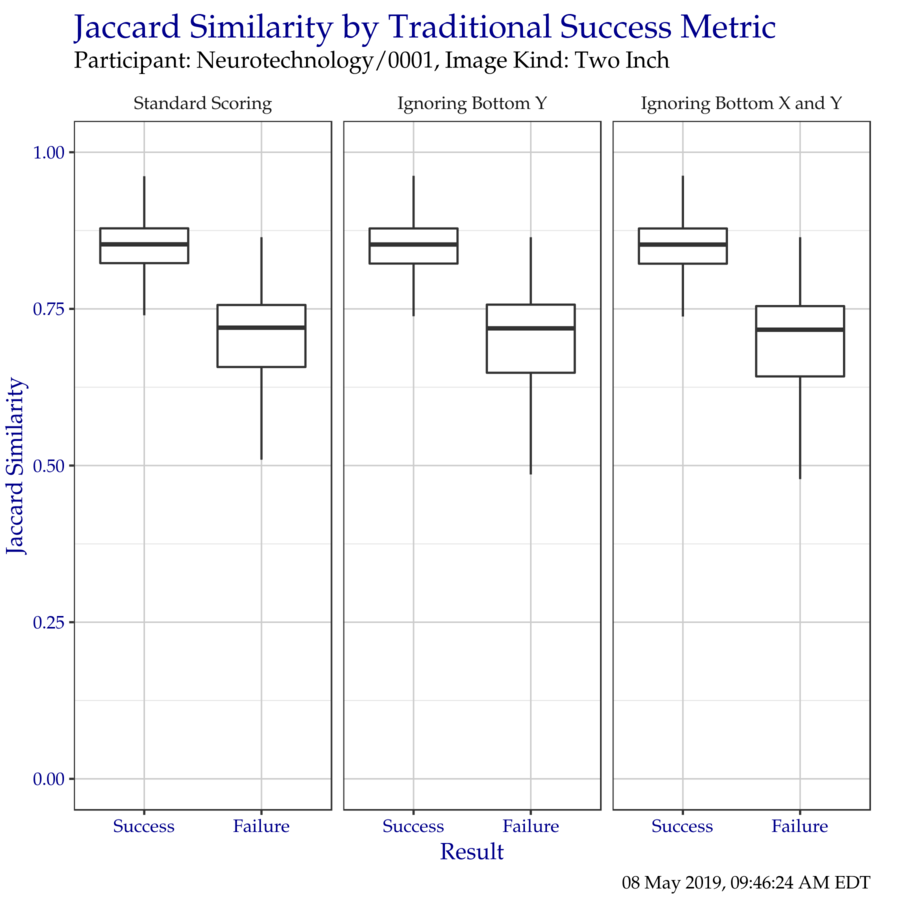
\includegraphics{/mnt/isiA01/evaluations/slapsegiii/analysis/intermediate/Neurotechnology/0001/full/Neurotechnology+0001_full_TwoInch_jaccard-by-success} 

}

\caption{Boxplot of Jaccard similarity indices as compared to the traditional success metrics. Outliers have been removed for clarity.}\label{fig:twoinch-jaccard-success}
\end{figure}

\begin{figure}

{\centering 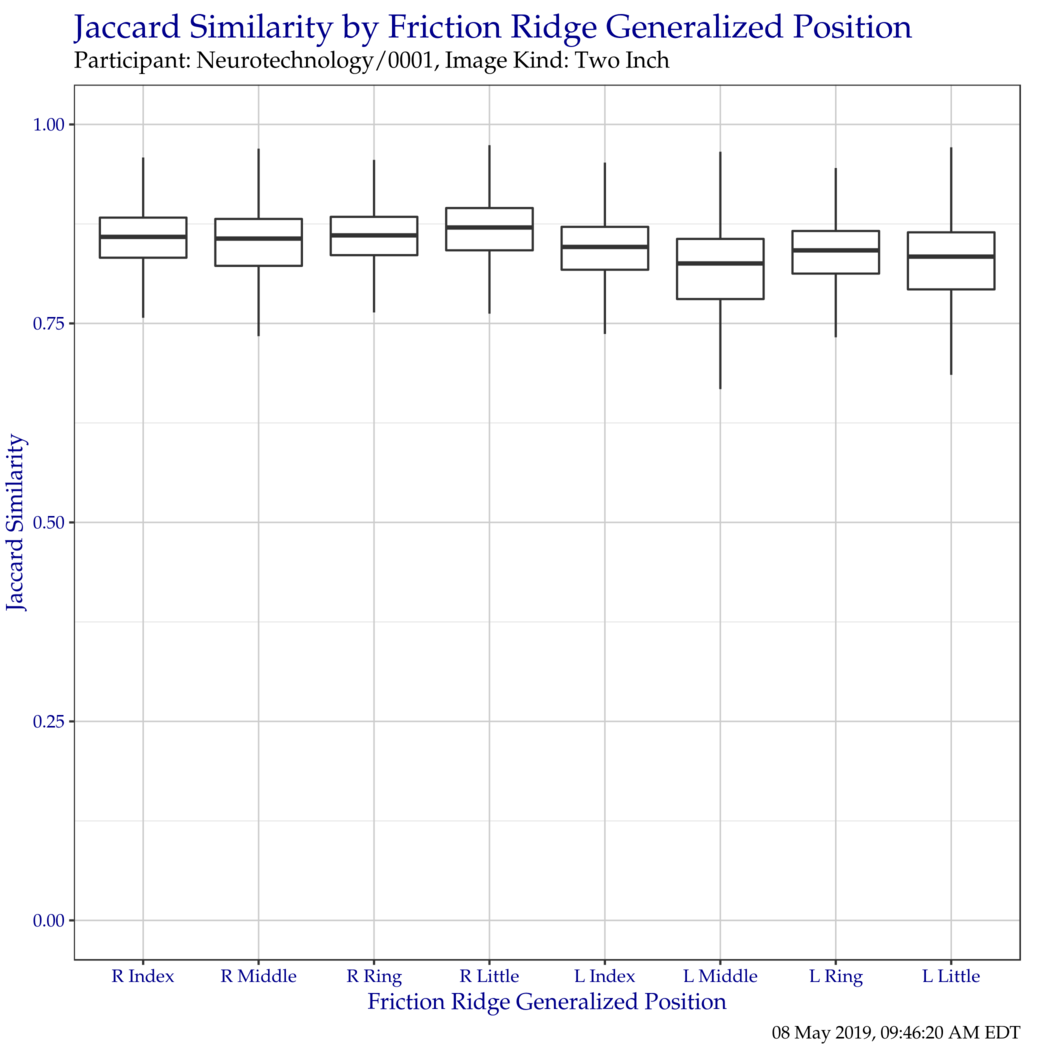
\includegraphics{/mnt/isiA01/evaluations/slapsegiii/analysis/intermediate/Neurotechnology/0001/full/Neurotechnology+0001_full_TwoInch_jaccard-by-frgp} 

}

\caption{Boxplot of Jaccard similarity indices for each friction ridge generalized position. Outliers have been removed for clarity.}\label{fig:twoinch-jaccard-frgp}
\end{figure}

\begin{table}[!h]

\caption{\label{tab:twoinch-per-subject-jaccard}For each subject, the percentage that at least \textit{Number of Fingers} fingers were segmented with a Jaccard index in the indicated range.}
\centering
\begin{tabular}{rlllllll}
\toprule
Number of Fingers & $\ge$0.5 & $\ge$0.6 & $\ge$0.7 & $\ge$0.8 & $\ge$0.9 & $\ge$0.95 & $\ge$0.98\\
\midrule
\rowcolor{gray!6}  1 & 99.9 & 99.9 & 99.9 & 99.7 & 45.6 & 2.5 & 0.1\\
2 & 99.8 & 99.8 & 99.8 & 99.3 & 20.9 & 0.2 & 0.0\\
\rowcolor{gray!6}  3 & 99.6 & 99.6 & 99.5 & 98.0 & 8.8 & 0.0 & 0.0\\
4 & 99.3 & 99.2 & 98.8 & 93.9 & 2.9 & 0.0 & 0.0\\
\rowcolor{gray!6}  5 & 95.8 & 95.8 & 95.7 & 86.2 & 0.6 & 0 & 0\\
6 & 95.6 & 95.6 & 95.1 & 75.9 & 0.1 & 0 & 0\\
\rowcolor{gray!6}  7 & 95.0 & 94.9 & 92.4 & 58.7 & 0.0 & 0 & 0\\
8 & 92.9 & 91.6 & 81.1 & 31.8 & 0 & 0 & 0\\
\bottomrule
\end{tabular}
\end{table}

\begin{table}[!h]

\caption{\label{tab:twoinch-per-frgp-jaccard}For all subjects, percentage that a particular friction ridge generalized position was segmented with a Jaccard index in the indicated range.}
\centering
\begin{tabular}{lllllll}
\toprule
Finger & 0-0.5 & 0.5-0.6 & 0.6-0.7 & 0.7-0.8 & 0.8-0.9 & 0.9-1.0\\
\midrule
\addlinespace[0.3em]
\multicolumn{7}{l}{\textbf{Right}}\\
\rowcolor{gray!6}  \hspace{1em}Index & 0.4 & 0.0 & 0.6 & 8.6 & 77.8 & 12.6\\
\hspace{1em}Middle & 0.7 & 0.1 & 1.8 & 14.0 & 72.4 & 11.0\\
\rowcolor{gray!6}  \hspace{1em}Ring & 0.3 & 0.0 & 0.5 & 7.6 & 79.4 & 12.2\\
\hspace{1em}Little & 0.4 & 0.1 & 0.8 & 7.6 & 70.5 & 20.6\\
\addlinespace[0.3em]
\multicolumn{7}{l}{\textbf{Left}}\\
\rowcolor{gray!6}  \hspace{1em}Index & 0.4 & 0.0 & 0.6 & 14.5 & 77.6 & 6.9\\
\hspace{1em}Middle & 1.4 & 0.3 & 4.1 & 28.2 & 63.1 & 2.9\\
\rowcolor{gray!6}  \hspace{1em}Ring & 0.6 & 0.2 & 1.4 & 16.3 & 77.3 & 4.2\\
\hspace{1em}Little & 0.8 & 0.5 & 3.1 & 24.0 & 66.5 & 5.1\\
\bottomrule
\end{tabular}
\end{table}

\begin{table}[!h]

\caption{\label{tab:twoinch-per-hand-all-jaccard}Percentage of segmentation obtaining a Jaccard index in the indicated ranges, by hand, for combinations of all eight fingers of a TwoInch slap.}
\centering
\begin{tabular}{llllllll}
\toprule
Fingers & $\ge$0.5 & $\ge$0.6 & $\ge$0.7 & $\ge$0.8 & $\ge$0.9 & $\ge$0.95 & $\ge$0.98\\
\midrule
\addlinespace[0.3em]
\multicolumn{8}{l}{\textbf{Right}}\\
\rowcolor{gray!6}  \hspace{1em}Any & 100.0 & 100.0 & 100.0 & 99.4 & 35.7 & 1.8 & 0.0\\
\hspace{1em}At Least Two & 99.9 & 99.9 & 99.9 & 98.1 & 14.3 & 0.1 & 0.0\\
\rowcolor{gray!6}  \hspace{1em}At Least Three & 99.7 & 99.6 & 99.4 & 92.1 & 5.2 & 0.0 & 0.0\\
\hspace{1em}All Four & 98.8 & 98.5 & 95.0 & 66.8 & 1.1 & 0.0 & 0.0\\
\addlinespace[0.3em]
\multicolumn{8}{l}{\textbf{Left}}\\
\rowcolor{gray!6}  \hspace{1em}Any & 99.9 & 99.9 & 99.9 & 96.0 & 15.6 & 0.4 & 0.1\\
\hspace{1em}At Least Two & 99.8 & 99.8 & 99.6 & 89.2 & 3.0 & 0.0 & 0.0\\
\rowcolor{gray!6}  \hspace{1em}At Least Three & 99.4 & 99.3 & 98.3 & 74.8 & 0.4 & 0.0 & 0.0\\
\hspace{1em}All Four & 97.8 & 96.9 & 88.8 & 43.7 & 0.1 & 0.0 & 0.0\\
\bottomrule
\end{tabular}
\end{table}

\begin{table}[!h]

\caption{\label{tab:twoinch-per-hand-index-middle-jaccard}Percentage of segmentation obtaining a Jaccard index in the indicated ranges, by hand, for combinations of index and middle fingers of a TwoInch slap.}
\centering
\begin{tabular}{llllllll}
\toprule
Fingers & $\ge$0.5 & $\ge$0.6 & $\ge$0.7 & $\ge$0.8 & $\ge$0.9 & $\ge$0.95 & $\ge$0.98\\
\midrule
\addlinespace[0.3em]
\multicolumn{8}{l}{\textbf{Right}}\\
\rowcolor{gray!6}  \hspace{1em}Either Index or Middle & 99.8 & 99.8 & 99.8 & 97.5 & 19.8 & 0.7 & 0.0\\
\hspace{1em}Both Index and Middle & 99.1 & 99.0 & 96.7 & 76.3 & 3.7 & 0.0 & 0.0\\
\addlinespace[0.3em]
\multicolumn{8}{l}{\textbf{Left}}\\
\rowcolor{gray!6}  \hspace{1em}Either Index or Middle & 99.8 & 99.8 & 99.6 & 91.1 & 9.2 & 0.3 & 0.1\\
\hspace{1em}Both Index and Middle & 98.5 & 98.2 & 93.6 & 59.5 & 0.6 & 0.0 & 0.0\\
\bottomrule
\end{tabular}
\end{table}

\begin{table}[!h]

\caption{\label{tab:twoinch-per-hand-index-middle-ring-jaccard}Percentage of segmentation obtaining a Jaccard index in the indicated ranges, by hand, for combinations of index, middle, and ring fingers of a TwoInch slap.}
\centering
\begin{tabular}{llllllll}
\toprule
Fingers & $\ge$0.5 & $\ge$0.6 & $\ge$0.7 & $\ge$0.8 & $\ge$0.9 & $\ge$0.95 & $\ge$0.98\\
\midrule
\addlinespace[0.3em]
\multicolumn{8}{l}{\textbf{Right}}\\
\rowcolor{gray!6}  \hspace{1em}Any & 99.9 & 99.9 & 99.9 & 99.0 & 25.7 & 1.0 & 0.0\\
\hspace{1em}At Least Two & 99.7 & 99.7 & 99.6 & 94.6 & 8.3 & 0.0 & 0.0\\
\rowcolor{gray!6}  \hspace{1em}All Three & 99.0 & 98.8 & 96.1 & 71.8 & 1.8 & 0.0 & 0.0\\
\addlinespace[0.3em]
\multicolumn{8}{l}{\textbf{Left}}\\
\hspace{1em}Any & 99.9 & 99.9 & 99.8 & 94.4 & 12.2 & 0.3 & 0.1\\
\rowcolor{gray!6}  \hspace{1em}At Least Two & 99.5 & 99.5 & 99.0 & 83.3 & 1.7 & 0.0 & 0.0\\
\hspace{1em}All Three & 98.2 & 97.8 & 92.2 & 54.3 & 0.1 & 0.0 & 0.0\\
\bottomrule
\end{tabular}
\end{table}


\end{document}
